% !TEX root = index.tex
\section{How Curved is a Potato?}
\epigraph{The heart of mathematics consists of concrete examples and concrete problems. Big general theories are usually afterthoughts based on small but profound insights; the insights themselves come from concrete special cases.}{Paul Halmos}

Surfaces are much more varied than curves. The standard examples of surfaces are a plane, a cylinder, a saddle, a sphere, a torus etc. It is hard to come up with a single number that completely describes how curved these objects are. So the better question is what's the right amount of information we need to quantify curvature of these objects?

\subsection{Defining Curvature for Graphs}
For us a surface $S$ is just a connected smooth 2-dimensional subset of $\R^3$. We want our surfaces to be nice, with no sharp edges and no self-intersections.\footnote{A surface is a connected smooth 2-dimensional submanifold of $ \R^n$ without a boundary.}

It is unclear that we can use an approximating sphere or something similar to define curvature. But we know that for curves the curvature measures the \emph{quadratic behavior} of the curve. As with curves, we'll start by analyzing graphs of functions $f(x,y):\R^2 \rightarrow \R$
\begin{align*}
  S = \{ (x,y,z) : z = f(x,y)\}
\end{align*}
We'll further assume that $p=(0,0)$ is a critical point of $f(x,y)$ i.e.
\begin{align*}
   f_x(p) = 0 = f_y(p)
\end{align*}
Our experience with curves suggests that we should define the curvature of $ S$ at $ p$ to be the triple
$$\kappa \stackrel{?}{=} (f_{xx}(p), f_{xy}(p), f_{yy}(p))$$
but there is a catch.






\subsection{The Catch}
We can rotate $ \R^3$ about the $ z-\mbox{axis}$ and the new surface $ S'$ will still satisfy the properties mentioned above. The new surface $ S'$ will be described by a completely different function $ g(x,y)$ and the second derivatives of $ g(x,y)$ will be different from those of $ f(x,y)$. However, the curvatures of $ S$ and $S'$ should be the same. This problem did not arise for curves because there is no way to {rotate $ \R^2$ about the $ y$-axis}.

\begin{figure}[H]
  \centering
  \begin{subfigure}[t]{0.495\textwidth}
    \centering
    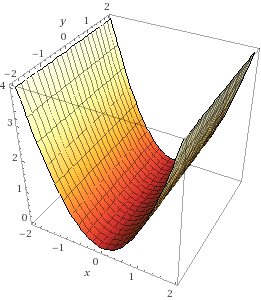
\includegraphics[width=6cm]{parabola1}
    \caption{$ f(x,y) = x^2 $ has second derivatives $ (2,0,0)$}
  \end{subfigure}
  \begin{subfigure}[t]{0.495\textwidth}
    \centering
    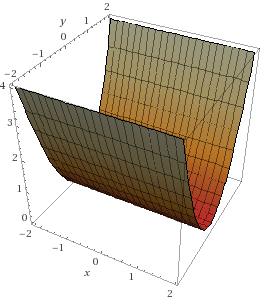
\includegraphics[width=6cm]{parabola2}
    \caption{$ f(x,y) = y^2 $ has second derivatives $ (0,0,2)$}
  \end{subfigure}
  \caption{The two surfaces are related to each other by a rotation about the $ z$-axis but they have very different second derivatives.}
\end{figure}

\begin{ques}
  \label{ques:paraboloid}
  Rotate the parabolic cylinder $z=x^2$ about the  $z$-axis by an angle $\theta$ in the counter-clockwise direction. Describe the new surface as the graph of some function $f_{\theta}(x,y)$. Find the second derivatives of $f_{\theta}(x,y)$.
\end{ques}






\subsection{Rotations and Second Derivatives}
We need to understand how the second derivatives change when we rotate the $ xy$-plane about the $ z$-axis. There are two tricks to do this efficiently.\footnote{In order to avoid clutter we'll stop writing the $ (p)$. All the derivatives are being taken at the critical point $p = (0,0)$.}

\begin{description}
  \item{\bf Trick \#1} Instead of analyzing the second derivatives we analyze the degree 2 Taylor polynomial
  \begin{align*}
    2f(x,y) \approx 2f(p) + f_{xx}\cdot {x^2} + 2f_{xy} \cdot {xy} + f_{yy} \cdot {y^2}
  \end{align*}

  \item{\bf Trick \#2} We rewrite the degree 2 Taylor polynomial in matrix form
  \begin{align*}
    2f(x,y)
    &\approx 2f(p) +
    \begin{bmatrix} x & y \end{bmatrix}
    \begin{bmatrix}
      f_{xx} & f_{xy} \\
      f_{xy} & f_{yy}
    \end{bmatrix}
    \begin{bmatrix} x \\ y \end{bmatrix}
  \end{align*}
\end{description}
The rotation or the reflection of the $ xy$-plane about the $z$-axis is a linear transformation and hence can be described by some orthogonal matrix $ A$
\begin{align*}
  \begin{bmatrix} x \\ y \end{bmatrix}
    &= A
  \begin{bmatrix} x' \\ y' \end{bmatrix}
\end{align*}
Plugging this in the right hand side of the Taylor polynomial we get
\begin{align}
  \nonumber
  2f(x,y)
  &\approx 2f(p) + f_{xx}{x^2} + 2f_{xy} {xy} + f_{yy}{y^2} \\
  \nonumber
  &= 2f(p) +
  \begin{bmatrix} x & y \end{bmatrix}
  \begin{bmatrix}
    f_{xx} & f_{xy} \\
    f_{xy} & f_{yy}
  \end{bmatrix}
  \begin{bmatrix} x \\ y \end{bmatrix} \\
    \label{eq:Hessian}
    &= 2f(p) +
    \begin{bmatrix} x' & y' \end{bmatrix} A^T
    \begin{bmatrix}
      f_{xx} & f_{xy} \\
      f_{xy} & f_{yy}
    \end{bmatrix}
    A \begin{bmatrix} x' \\ y' \end{bmatrix}
\end{align}
Notice that the right hand side is still quadratic, and not surprisingly this is \textbf{the Taylor approximation of $ f$ in terms of $ (x',y')$}.
\begin{ques}
  Let $A$ denote reflection of the $xy$-plane about the line $x=y$.
  \begin{enumerate}
    \item Express $A$ as a $2 \times 2$ matrix.
    \item Expand the right hand side of \eqref{eq:Hessian} for this $A$ and verify that this is indeed the degree 2 Taylor approximation in the new variables.
  \end{enumerate}
\end{ques}
\begin{ques}
  Suppose that $A = \begin{bmatrix} m & 0 \\ 0 & n \end{bmatrix}$ where $m,n$ are non-zero real numbers. This linear transformation corresponds to scaling the $x,y$ axes by $m,n$ respectively. Expand the right hand side of \eqref{eq:Hessian} for this $A$ and verify that this is indeed the degree 2 Taylor approximation in the new variables.
\end{ques}
\begin{definition}
  The matrix $\begin{bmatrix} f_{xx} & f_{xy} \\ f_{xy} & f_{yy} \end{bmatrix}$ is called the \textbf{Hessian} of $ f$, denoted $ \hess(f)(x,y)$.
\end{definition}
\begin{thm}
  \label{thm:change_of_coords_Hessian}
  At a critical point $p$, if the coordinates change according to the linear transformation $$\begin{bmatrix} x \\ y \end{bmatrix} = A \begin{bmatrix} x' \\ y' \end{bmatrix}$$ then the Hessian $ \hess(f)$ changes as
  \begin{align}
    \label{eq:2-tensor}
    \begin{bmatrix}
      f_{x'x'} & f_{x'y'} \\
      f_{x'y'} & f_{y'y'}
    \end{bmatrix}
      &=
       A^T
      \begin{bmatrix}
        f_{xx} & f_{xy} \\
        f_{xy} & f_{yy}
      \end{bmatrix}
      A
  \end{align}
  We say that $\hess(f)$ is a 2-tensor at a critical point.
\end{thm}
\begin{remark}
  The assumption that we're at a critical point i.e. $ f_x = 0 = f_y$ is extremely crucial here and cannot be dropped. If, for example, we further had $ f_x = 0 = f_y$ and $ f_{xx} = 0 = f_{xy} = f_{yy}$ then we will get a similar change of coordinate rule for the third derivatives, which will be a 3-tensor.
\end{remark}












\subsection{The Curvatures}
The Curvature(s) should be \emph{invariants} of the matrix $ \hess(f)$ which remain unchanged when we apply the transformation \eqref{thm:change_of_coords_Hessian} where $ A$ is either a rotation or a reflection. When $A$ is one of these we further have $A^T = A^{-1}$ so that
\begin{align*}
  \begin{bmatrix}
    f_{x'x'} & f_{x'y'} \\
    f_{x'y'} & f_{y'y'}
  \end{bmatrix}
    &=
     A^{-1}
    \begin{bmatrix}
      f_{xx} & f_{xy} \\
      f_{xy} & f_{yy}
    \end{bmatrix}
    A
\end{align*}
We say that $\hess(f)(x,y)$ and $\hess(f)(x',y')$ are {\bf similar} or {\bf conjugate} to each other i.e. they represent the same linear transformation. If two matrices represent the same linear transformation then they have the same \emph{determinant} and \emph{trace}.
\begin{ques}
  Let $A$ be an $n\times n$ matrix and let $P$ be an invertible $n \times n$ matrix. Prove that
  \begin{align*}
    \det A = \det (P A P^{-1}) \mbox{ \: and \: }\tr A = \tr(P A P^{-1})
  \end{align*}
\end{ques}
We now have well defined notions of curvature which remain unchanged when we rotate or reflect the $xy$-plane.
\begin{definition}
  If $ S$ is the graph of a smooth function $ f(x,y)$ satisfying $ f_x(p) = 0 = f_y(p)$ then
  \begin{enumerate}
    \item The \textbf{Mean Curvature} of $ S$ at $ p$ is defined to be
    \begin{align*}
      H = \tr(\hess(f))/2 = (f_{xx} + f_{yy})/2
    \end{align*}
    \item The \textbf{Gaussian Curvature} of $ S$ at $ p$ is defined to be \textbf{determinant}
    \begin{align*}
      K = \det(\hess(f)) = f_{xx}f_{yy} - f_{xy}^2
    \end{align*}
  \end{enumerate}
\end{definition}


\begin{ques}
  Go back to your computation in Question \ref{ques:paraboloid} and verify that the Gaussian and Mean curvatures for $z=f_\theta(x,y)$ do not depend on $\theta$.
\end{ques}

\begin{ques}
  For each of the following surfaces, find the second order Taylor polynomial, the Hessian, and the Mean and Gaussian curvatures at $(0,0)$.
  \begin{description}
    \item[The Perfect \textbf{Potato Chip}: ]  $ z = x^2 - y^2 $
    \item[Cylindrical Potato: ] $z = -\sqrt{r^2 - x^2} $
    \item[Spherical Potato: ] $z = -\sqrt{r^2 - x^2 - y^2}$
    \item[Parabolic Cylinder: ] $z =  x^2$
  \end{description}
  (You can use the estimate $-\sqrt{r^2 - \alpha} \approx -r + \frac{\alpha}{2r} $. This is called the \textbf{binomial approximation}.)
\end{ques}

\begin{remark}
  Although we're only analyzing critical points of graphs of functions, we can always rotate $ \R^3$ (which should not change curvatures) so that the surface looks like a graph near the point of interest, and the point becomes a critical point. As such, the above method defines curvature in all generality.
\end{remark}

\subsection{Appendix: Taylor approximation}
Taylor polynomials are a way to approximate functions by polynomials.
\begin{definition}
	The degree $ n$ \textbf{Taylor approximation} of a function $ f: \R \rightarrow \R$ at a point $ x=a$ is defined to be
	\begin{align*}
		f(a) + \dfrac{f'(a)}{1!} (x-a) + \dfrac{f''(a)}{2!} (x-a)^2 + \cdots + \dfrac{f^{(n)}(a)}{n!} (x-a)^n
	\end{align*}
	where $f^{(n)}(a)$ denotes the $ n^{th}$ derivative of $ f$ at $ a$.
\end{definition}
We're only interested in the degree 2 approximation at $ x=0$ i.e. $$ f(x)
	\approx f(0) + f'(0) x + f''(0) \frac{x^2}{2}$$
This generalizes to functions in multiple variables easily.
\begin{definition}
	The degree 2 or \textbf{second order Taylor approximation} of a function $ f: \R^2 \rightarrow \R$ at the point $ p=(0,0)$ is defined to be
	\begin{align*}
		f(x,y) \approx f(p) + f_x(p)\cdot x + f_y(p)\cdot y + f_{xx}(p)\cdot \frac{x^2}{2} + f_{xy}(p) \cdot xy + f_{yy}(p)\cdot \frac{y^2}{2}
	\end{align*}
	where $f_{*}(p)$ denotes the partial derivatives.\footnote{$f_{xy}$ has coefficient 1 instead of $1/2$ as it is secretly a sum of two terms $f_{xy}$ and $f_{yx}$ which happen to be equal for all twice differential functions.}
\end{definition}
\begin{ques}
	If $ f(x,y)$ is polynomial in 2 variables $x,y$ find it's the second order Taylor approximation at $(0,0)$.
\end{ques}
\begin{ques}
  Let $T_2(f)$ denote the degree 2 Taylor approximation of $f$ at $(0,0)$. Let $P$ denote the vector space of smooth functions $\R^2 \rightarrow \R$ and let $P_2$ denote the vector space of polynomials of degree $\le 2$ with real coefficients.
  \begin{enumerate}
    \item Show that $T_2$ defines a linear transformation $P \rightarrow P_2$.
    \item Further show that $T_2(T_2(f)) = T_2(f)$.
  \end{enumerate}
\end{ques}
Linear transformations $L$ which satisfy $L \circ L = L$ are called \textbf{projections}, and thus taking the degree 2 Taylor approximation is like projecting onto the space of degree 2 polynomials.











\subsection{Appendix: Orthogonal Transformations}
\begin{ques}$ $
  \begin{enumerate}
    \item Prove that every rotation of $\R^2$ about the origin is given by a linear transformation of the form
    \begin{align*}
      \begin{bmatrix}
        \cos \theta & -\sin \theta \\
        \sin \theta & \cos \theta
      \end{bmatrix}
    \end{align*}
    \item Prove that every reflection of $\R^2$ about a line passing through the origin is given by a linear transformation of the form
    \begin{align*}
      \begin{bmatrix}
        -\cos \theta & \sin \theta \\
        \sin \theta & \cos \theta
      \end{bmatrix}
    \end{align*}
    \item Prove that both reflections and rotations satisfy
    \begin{align*}
      A^{-1} = A^T
    \end{align*}
    \item Show that if $A$ is a $2 \times 2$ matrix satisfying $A^{-1} = A^T$ then $A$ is either a rotation or a reflection.
  \end{enumerate}
\end{ques}
In higher dimensions it is difficult to give explicit descriptions of rotations and reflections, instead we define \textbf{orthogonal matrices} to be the ones that satisfy $A^{-1} = A^T$. It is easy to show that orthogonal matrices preserve distances and angles and hence are the correct generalizations of rotations and reflections.
